\subsection{AGRC analysis}
\label{sec:agrc-analysis}

%In order to statically determine the worst case memory consumption of a
%program targeting TP-JOP, one needs to analyze codes generated from both
%CNs and JDNs. The compiler is able to trivially determine the maximum
%memory footprint required for executing CN codes from any given SystemJ
%programs [] since there is no dynamic memory allocation required for
%executing this code. On the other hand, the data-flow analysis for JDNs
%is more intricate since it needs to analyze the original AGRC in order
%to retrieve the dependency edges, which are lost after splitting CNs and
%JDNs from the AGRC. We devote this section to illustrate this analysis
%technique.


AGRC is a \textit{directed graph} of tuple $G =(V,E)$, where $V$ is the
set of vertices (nodes of AGRC) and $E$ is the set of ordered pairs of
vertices. Each edge $e = (v_i,v_j), \forall e \in E, v_i \in V, v_j \in
V$ is a tuple denoting that the edge is directed from $v_i$ to $v_j$.
Then a lambda  function $\lambda:v \rightarrow E_i$, $E_i \subseteq E$,
maps \textit{each} vertex to a set of edge(s) where $\forall (v_i,v_j)
\in E_i, v_j = v$ and $E_i$ can be $\emptyset$. When $|E_i| = 1$ we call
$v_i$ \textit{must} be called before $v$ whereas when $|E_i| > 1$ we
call any $v_i \in E_i$ \textit{may} be called before $v$.

\begin{figure}[t!]
	\newsavebox{\codeone}
	\begin{lrbox}{\codeone}
		\begin{minipage}[b]{0.62\textwidth}
		\begin{lstlisting}[tabsize=1,basicstyle=\small\ttfamily,numbers=left]
(mList 
	(mNode JDN1 (Must Null) (May Null))
	(mNode JDN2 
		(Must (mNode JDN1 (Must Null) (May Null))) 
		(May Null))
	(mNode JDN3 
		(Must (mNode JDN1 (Must Null) (May Null))) 
		(May Null))
	(mNode JDN4 (Must Null)
		(May 
			(mNode JDN2 
				(Must (mNode JDN1 (Must Null) (May Null))) 
				(May Null))
			(mNode JDN3 
				(Must (mNode JDN1 (Must Null) (May Null))) 
				(May Null))))
		\end{lstlisting}
	\end{minipage}
	\end{lrbox}

	\centering
	\subfloat[An abstracted AGRC graph]{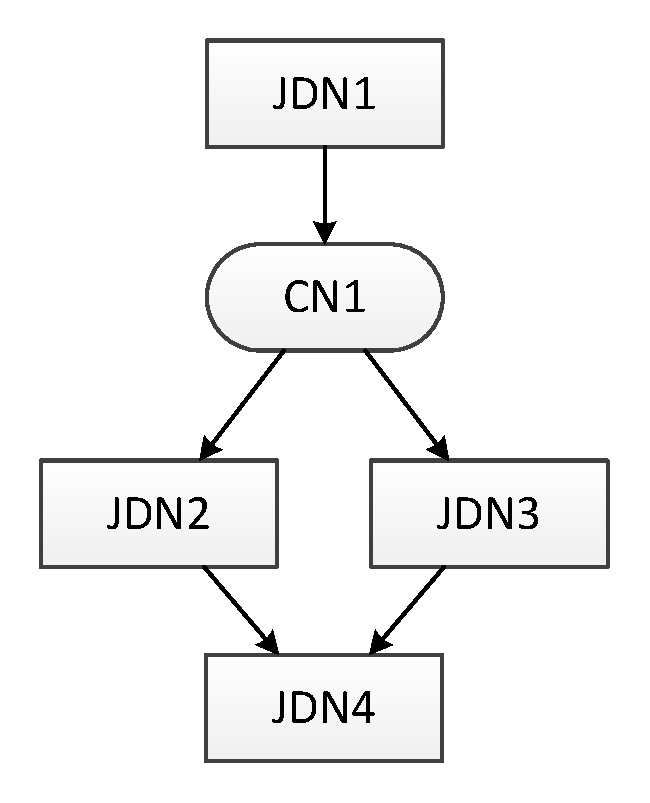
\includegraphics[scale=0.3]{may}
	\label{fig:aagrc}}
	\hspace{1.0cm}
	\subfloat[An output of the AGRC
	analysis]{\scalebox{0.8}{\usebox{\codeone}}\label{fig:tttt}}
	\caption{An example of AGRC analysis}
	\label{fig:maymust}
\end{figure}

In this section, we illustrate how a data-structure is obtained from the
AGRC, which contains \textit{may} and \textit{must} relationships
between the nodes. Consider a snippet of AGRC graph shown in
Figure~\ref{fig:aagrc}. Here, the root node, \texttt{JDN1}, has no
parents, which has an immediate child \texttt{CN1}. \texttt{CN1} then
forks two children, \texttt{JDN2} and \texttt{JDN3}, and finally both of
these JDNs have an identical child \texttt{JDN4}. This graph is then
given as an input to the algorithm, which performs the AGRC analysis
(Figure~\ref{fig:6c}). An output of the analysis a data-structure which
contains \textit{may} and \textit{must} relationships between the nodes
in AGRC graph. Figure~\ref{fig:tttt} shows an example of such
data-structure, which is a set of nodes called \texttt{mNode}.
\texttt{mNode} has three fields, a node name of type string,
\texttt{Must} of \texttt{mNode} and \texttt{May} of a set of
\texttt{mNode}.





%%% Local Variables:
%%% mode: latex
%%% TeX-master: "jgc"
%%% End:
